\documentclass[11.5pt]{sig-alternate} % sets document style to sig-alternate
% packages
% typesetting
%\usepackage{dirtytalk} % typset quotations easier (\say{stuff})
\usepackage{hanging} % hanging paragraphs
\usepackage[defaultlines=3,all]{nowidow} % avoid widows
\usepackage[pdfpagelabels=false]{hyperref} % produce hypertext links, includes backref and nameref
\usepackage{xurl} % defines url linebreaks, loads url package
\usepackage{microtype}
\usepackage{textgreek}
%\usepackage{textcomp}
%\newcommand{\texttildemid}{\raisebox{0.4ex}{\texttildelow}}
% layout
\usepackage{enumitem} % control layout of itemize, enumerate, description
\usepackage{fancyhdr} % control page headers and footers
\usepackage{float} % improved interface for floating objects
%\usepackage{multicol} % intermix single and multiple column pages
% language
\usepackage[utf8]{inputenc} % accept different input encodings
\usepackage[english]{babel} % multilanguage support
% misc
\usepackage{graphicx} % builds upon graphics package, \includegraphics
%\usepackage{lastpage} % reference number of pages
%\usepackage{comment} % exclude portions of text (?)
\usepackage{xcolor} % color extensions
\usepackage[backend=biber, style=apa]{biblatex} % sophisticated bibliographies % necessary for HTML to display author info and date on abstract page
\usepackage{csquotes} % advanced quotations, makes biblatex happy
\usepackage{authblk} % support for footnote style author/affiliation
% tables and figures
\usepackage{tabularray}
%\usepackage{array} % extend array and tabular environments
\usepackage{caption} % customize captions in figures and tables (rotating captions, sideways captions, etc)
%\usepackage{cuted} % allow mixing of \onecolumn and \twocolumn on same page
\usepackage{multirow} % create tabular cells spanning multiple rows
%\usepackage{subfigure} % deprecated, support for manipulation of small figures
%\usepackage{tabularx} % extension of tabular with column designator "x", creates paragraph-like column whose width automatically expands
%\usepackage{wrapfig} % allows figures or tables to have text wrapped around them
%\usepackage{booktabs} % better rules
% dummy text
%\usepackage{blindtext} % blind text dummy text
%\usepackage{kantlipsum} % Kant style dummy text
\usepackage{lipsum} %lorem ipsum dummy text
% other helpful packages may be booktabs, longtable, longtabu, microtype

\pagestyle{fancy} % sets pagestyle to fancy for fancy headers and footers

% header and footer
% modern way to set header image
\renewcommand{\headrulewidth}{0pt} % defines thickness of line under header
\renewcommand{\footrulewidth}{0pt} % defines thickness of line above header
\setlength\headheight{80.0pt} % sets height between top margin and header image, effectively moves page contents down
\addtolength{\textheight}{-80.0pt} % seems to affect the lower height. maybe only works properly if footer numbers enabled?
\fancyhf{}
\fancyhead[CE, CO]{
\includegraphics[width=\textwidth]{headerImage.png}}
% footer
%\fancyfoot[LE,LO]{Article Title Here \\ DOI: }% left footer article title and doi
%\fancyfoot[CE,CO]{{}} % center footer empty
%\fancyfoot[RE,RO]{\thepage} % right footer page numbers
%\pagenumbering{arabic} % arabic (1, 2, 3) numbering in footer

\hypersetup{colorlinks=true,urlcolor=blue} % sets link color to blue
\urlstyle{same} % sets url typeface to same as rest of text

% set caption and figure to italics, label bold, left align captions, does not transfer to HTML
\captionsetup{labelfont=bf, font={large, it}, justification=raggedright, singlelinecheck=false}
\renewcommand\theContinuedFloat{\alph{ContinuedFloat}}

%this next bit is confusing, but essentially changes the width of the abstract. Seems to have been copied from this https://tex.stackexchange.com/questions/151583/how-to-adjust-the-width-of-abstract
\let\oldabstract\abstract
\let\oldendabstract\endabstract
\makeatletter %changes @ catcode to enable modification (in parsep)
\renewenvironment{abstract} %alters the abstract environment
{\renewenvironment{quotation}%
               {\list{}{\addtolength{\leftmargin}{1em} % change this value to add or remove length to the the default ?
                        \listparindent 1.5em%
                        \itemindent    \listparindent%
                        \rightmargin   \leftmargin%
                        \parsep        \z@ \@plus\p@}%
                \item\relax}%
               {\endlist}%
\oldabstract}
{\oldendabstract}
\makeatother %changes @ catcode to disable modification

% checks
% italics
% links
% dashes
% tildes
\begin{document}

\title{A Program Like Any Other…Like None Other: Sustaining a Laboratory Science Technology Program for Deaf and Hard-of-Hearing Students}

\author[1]{\large \color{blue} Todd Pagano}
\author[1]{\large \color{blue} Annemarie D. Ross}
\author[2]{\large \color{blue} George J. O'Neill}


\affil[1]{National Technical Institute for the Deaf/ Rochester Institute of Technology}
\affil[2]{American Chemical Society}
\toappear{}

\maketitle
\begin{@twocolumnfalse} 
\begin{abstract}
\item 
\begin{large}
\textit{A goal of the Laboratory Science Technology program at the National Technical Institute for the Deaf, a college of Rochester Institute of Technology, is to produce graduates with strong foundations in applied science, hands-on laboratory applications, and “soft skills” necessary for competitive employment as laboratory technicians. Graduates of the program earn Associate degrees, and if qualified, transition to related baccalaureate programs. Those who finish either an Associates of Occupational Science or Associates of Applied Science degree programs tend to go to work in the chemical, biological, biotechnology, pharmaceutical, environmental, forensic, industrial, and food analysis fields. At first glance, the LST program appears to be a typical chemical technology program similar to many others. However, it is the only one of its kind in the world. In order to achieve its successes it had to overcome unique challenges because it serves a large and unique population of deaf and hard-of-hearing students. Program challenges include enrollment, staffing and funding, and students/graduates finding cooperative works experiences/jobs. Still, through the use of outreach to future students, industrial alliances, curricular modifications, and other unique features, the program in now sustainable and growing.} 

\end{large}     
\end{abstract}
\end{@twocolumnfalse}

%% ABSTRACT

%% AUTHOR INFORMATION

\textbf{*Corresponding Author, Todd Pagano}\\
\href{mailto:tepnts@rit.edu}{(tepnts@rit.edu)}\\
\textit{Submitted December 17, 2013}\\
\textit{Accepted December 17, 2013}\\
\textit{Published Online December 17, 2013}\\
\textit{DOI: 10.14448/jsesd.04.0002}\\

\pagebreak
\clearpage
\section*{INTRODUCTION}
\begin{large}
In 2010 the United States Bureau of Labor Statistics (BLS) reported that the future looks bright for qualified science technicians who are seeking jobs. This is especially true for “graduates of applied science technology programs who are well trained on equipment used in industrial and government laboratories and production facilities”. (BLS, 2010-11) Two of the major reasons for the bright outlook are the increased rate of retirement of incumbent technicians and the serious lack of numbers of qualified replacements for them. This is the situation, today, for many of the 66,100 jobs (BLS, 2010-11) held by chemical laboratory technicians who are employed mostly in the basic chemical, R\&D services and pharmaceutical manufacturing industries. (BLS, May, 2010) Hofstader and Chapman (1997) of the American Chemical Society (ACS) anticipated this shortage of these essential workers in the late 1990’s. In their seminal report they called for the nation’s chemistry-based technology programs to rise and meet the challenge by increasing their output of well-trained laboratory technicians.(Hofstader \& Chapman, 1997)

The Laboratory Science Technology (LST) program at the National Technical Institute for the Deaf (NTID) at Rochester Institute of Technology (RIT) in Rochester, NY has taken the challenge to produce industry-ready chemical technicians seriously. The program was designed from an industry perspective and began educating students in 2002. Today, the program enrolls over 50 deaf and hard-of-hearing students, has over 75 alums, boasts a 100\% cooperative work experience (co-op)/internship placement rate, and nears a yearly 100\% rate of graduates who either gain employment as technicians or continue their education in higher degrees after completion of the LST program. Of the students who choose to continue their education, about 85\% persist to earning their baccalaureate. To date, the young program has produced 5 graduates who have gone on to complete Master’s degrees.

Nearly all chemical technology programs face challenges; including these critical issues outlined in a 2004 whitepaper on issues and effective practices of chemical technology programs (ChemTechLinks, 2006):
\begin{itemize}
    \item Alliances among industry, academia, community, and government
    \item Recruitment, retention, and placement
    \item National curriculum benchmarks and graduate skills assessments
    \item Faculty resources
    \item Incorporating updated technology and relevant subject matter into curricula
    \item Community awareness of the chemical technology profession
    \item Employability skills
    \item Relationships to grades K–12
    \item Industrial experiential learning opportunities
\end{itemize}

The LST program is not immune to many of these same challenges that other chemical technology programs face, but has found creative ways to circumvent some of these issues. As a result, he LST program can appear to be a quality chemical technology program like any other, but due to the unique population of deaf and hard-of-hearing students that it serves, it is a program like none other.

\subsection*{The College}
On June 14, 1965 President Lyndon B. Johnson created NTID when he signed a bill to promote the employment of individuals who are deaf or hard-of-hearing by providing them with technical and professional education opportunities. Today, NTID and its host school, RIT, have successfully collaborated to form the largest technical college in the world for educating deaf and hard-of-hearing students. The 1,500 or so students who have come from all 50 states and other countries can choose from programs that lead to associate’s, bachelor’s, master’s, and doctoral degrees in computing and information sciences, engineering, business, imaging sciences, liberal arts, and science. NTID provides unique services in a portion of faculty who are fluent in sign language, note takers, real-time captionists (voice to text translators), content area tutors, academic advisors, and the world’s largest group of college/university sign language interpreters.

\subsubsection*{On The Eve of a New Career}
Upon returning to Rochester, N.Y in 2002 I knew that I wanted to make a significant contribution to the education of students by making science as interesting, relevant, and rewarding as it was to me. What did I know about the world’s largest technological college for deaf and hard-of-hearing students? Not much. What did I know about communicating with deaf and hard-of-hearing students? Even less. What I did know was that these students should have the same chance for receiving a quality chemistry-based education and obtaining meaningful careers in the field, regardless of whether they could hear or not.

Ten years later, the program is thriving. In many ways, it is a program like any other– students discussing molecular bonding, solving stoichiometric problems, and operating analytical instrumentation. But it is also a program like no other– where all students are deaf or hard-of-hearing. I used my newly acquired skills in sign language, in conjunction with visuals, to communicate chemical information in the classroom and laboratory. I have seen these students embrace chemistry as I do, and become productive and valued members of the profession. I am extremely proud to be at the helm of program that seems to be as rewarding to me as it is to the students.
\\— Todd Pagano, Ph.D. Associate Professor \\(NTID/RIT) and LST Program Director

\subsection*{The Financial Picture}
When President Johnson created NTID, he also provided a commitment by the federal government to provide critical support through the Department of Education (DoE). Today, DoE contracts with RIT and provides a federal subsidy that tops \$60 million per year in order to enable NTID to provide quality post-secondary educational opportunities for individuals who are deaf and hard-of-hearing. Furthermore, many of NTID’s students receive tuition and other financial support from their respective state vocational rehabilitation agencies.

\subsection*{The Program}
While NTID marked its 40th anniversary, the LST program, which is one of the newer programs on the RIT campus, celebrated its 5th anniversary during the 2006-2007 academic year. After evaluating the market needs for laboratory technicians, the program was built with an industry perspective that is heavily focused on meeting the projected demand for skilled laboratory technicians. As mentioned, Hofstader \& Chapman (1997) also saw a strong need for greater numbers of well-trained chemical laboratory technicians. The overarching objective of LST’s faculty is to produce graduates with strong foundations in chemistry (fundamental, analytical, \& organic), biology, instrumental analysis, laboratory mathematics, laboratory applications, and requisite “soft skills”, so that they are able to gain employment in a competitive job market and/or continue their education in higher degree tracks.

The program’s curriculum has several features that help it to stand out against traditional post-secondary programs. A requirement for graduation is the successful completion of a 10-week co-op/internship anywhere in the country. Also, the unique six-part Laboratory Applications course series, which transcends covering traditional technical information by teaching some of the “soft skills” (i.e. effective communication strategies, ethics, and working as a valued member of a team), is an integral part of the program. Furthermore, the LST program takes it seriously when BLS says that there will be good job opportunities for those who are “well trained on equipment used in industrial and government laboratories and production facilities.” (BLS, 2010-11) A major strength of the program that pleases employers is the hands-on training that students get, specifically through the well-equipped and state-of-the-art instrumentation laboratory. These program features, combined with the solid technical knowledge and bench skills that are emphasized in the core courses, are paramount to assuring that LST graduates successfully transition from students to productive members of the technician workforce.

The student population in the LST program is truly unique. All of the program’s students, by nature of their deafness, belong to an underrepresented class in the field- while a majority of the students have also been consistently female (about 70\%). In addition, about one-third of the program’s students are from traditionally underrepresented groups (Latino, Native American, and African American). Graduates can achieve Associate in Occupational Studies (A.O.S.) and Associate in Applied Science (A.A.S.) degrees, and if qualified, can transition to related baccalaureate programs in chemistry, environmental science, or biotechnology studies at other colleges of RIT. These articulation agreements between NTID and RIT can be a major incentive for students who enroll in the LST program wanting to pursue a B.S degree. Those who finish either an A.O.S. or A.A.S. degree program, tend go to work in the chemical, biological, biotechnology, pharmaceutical, environmental, forensic, industrial, and food analysis fields.

Through the practical and applied focus of the program, deaf and hard-of-hearing LST students benefit from a hands-on curriculum with a focus on the use of analytical instrumentation and “bench skills” so that graduates are prepared to enter the workforce and immediately contribute to their host laboratory. Inasmuch as it is anticipated that graduates of the program might face communication, cultural, and attitudinal barriers in their future workplace, the LST program’s goal is to give its students a competitive advantage by ensuring that they are well-trained in the laboratory skills that are industry standards. The LST program recently received American Chemical Society (ACS) recognition by being the 15th Chemical Technology program to be awarded Program Approval. The program has been discussed in many media outlets, including several times in Chemical \& Engineering News (Amato, 2006; Huber, 2012; Hunt, 2007).

\subsubsection*{Synopsis of the LST Program}
The success of the LST program is largely due to the fact that it was built after evaluating industry’s needs for laboratory technicians. The program produces graduates with strong foundations in chemistry, biology, and mathematics. Students must also complete a cooperative work experience/internship anywhere in the country as part of their graduation requirements. Students have worked with Eastman Kodak, Novartis Pharmaceuticals, Stanford University, FDA, and NOAA- to name but a few organizations. A flagship of the program’s curriculum involves a newly renovated, well-equipped, and modern instrumentation laboratory.

The LST program has hosted four Presidents of the American Chemical Society, executives from international science companies, and prominent deaf scholars. The program has been written up several times in Chemical \& Engineering News and continues to grow at a rapid rate. However, nothing speaks to its success more than the number of deaf and hard-of-hearing students that have obtained a top-notch chemical education through enrollment in the program.

\subsection*{Recent Success Stories}
The following are a few important ways to measure the success of a technical academic program such as LST.
\begin{enumerate}[label=\Alph*)]
    \item \textit{Student Acceptance}
    \begin{sloppypar}Each year approximately 40 NTID students apply for admission to the LST program for about 25 openings. Due to logistical constraints of faculty headcount and limited laboratory space, the program can only accommodate about 50 total students in the program at any one time. Of freshmen who are accepted each year, about 60\% persevere to graduation. This rate is favorable compared to the 2009 national average of 29\% for students who persist to graduation, hearing or deaf. (NCHEMS, 2009)\end{sloppypar}
    \item \textit{Graduates Finding Jobs}
    \begin{sloppypar}For LST graduates, the rate for successfully finding jobs has recently reached 100\% and compares to the nearly 92\% reported rate for all NTID graduates in the past 5 years (National Technical Institute for the Deaf, 2011). This achievement is due in large to the hands-on laboratory skill development, the focus on “soft skills”, success graduates have while working for their co-op employers, and the tireless efforts of the faculty in assisting their graduates in reaching out to potential employers.\end{sloppypar}
    \item \textit{Professional Recognition}
    \begin{sloppypar}During its young existence, the LST program, faculty, and students have received positive recognition from professional organizations.\end{sloppypar}
    \begin{enumerate}
        \item[1.] The ACS has recognized dozens of LST students with “Chemical Technology Student Recognition Awards” for their “high level of performance in the laboratory and the classroom, excellent communication skills, integrity, and reliability.”
        \item[2.] In June 2006, an LST student was recognized as the sole recipient of the Wo\-men’s Chemist Committee’s (a committee of the American Chemical Society) “Overcoming Challenges Award”. This student received her award in September 2006 at the ACS national meeting in San Francisco, CA.
        \item[3.] The LST program has been featured in university, local, and national media. A notable distinction was being featured in an article published in Chemical \& Engineering News. (Amato, 2006)
        \item[4.] The LST program has recently been approved by the ACS Chemical Technology Program Approval Service (CTPAS). The program has been certified for 2009-2014.
        \item[5.] To date, the program has experienced visitations from four different active presidents of the ACS.
        \item[6.] Deaf and hard-of-hearing students from the program have participated in undergraduate research, and have disseminated the results of their work at various local and national symposia.
        \item[7.] Deaf and hard-of-hearing students from the program have participated in undergraduate research, and have disseminated the results of their work at various local and national symposia.
    \end{enumerate}
    \item \textit{Attracting Funding}
    \begin{sloppypar}In a field where one piece of equipment, such as a gas chromatographer-mass spectrometer (GC-MS), can cost over \$100,000, seeking funding can be a significant hurdle to a program’s success. Government and private agencies support initiatives to enhance unique educational and training opportunities for deaf and hard-of-hearing students. The LST program has benefited from securing funding for initiatives related to professional development for students, pedagogical advancements, and equipment. \end{sloppypar}
    \begin{enumerate}
        \item[1.] \underline{Student Professional Development}
        \begin{sloppypar}In the Fall of 2004, the program received funding from an anonymous donor, the ACS’s Committee on Chemists with Disabilities, and RIT to help cover the travel costs for about 40 students to attend sessions specifically designed for deaf and hard-of-hearing chemical professionals at the ACS Northeast Regional Meeting held in Rochester, NY. A highlight of this experience was the students’ participation in a focused career development workshop. This conference provided a mechanism for deaf and hard-of-hearing professionals and future professionals to gather and share experiences, get advice, and ask questions about their field. The students got a taste of the many resources, benefits, and professional development opportunities that a professional organization has to offer.
        
        Students have also received funding from the Rochester Section of the American Chemical Society’s Undergraduate Research Travel Award to attend national symposia. Through donations organized by the college’s Development Office, funds have been provided to support a LST student club. Students can also receive stipends/support from grants that faculty receive for research initiatives. \end{sloppypar}
        \item[2.] \underline{Pedagogical Advances}
        \begin{sloppypar}The program has also benefited from receiving institutional grants to explore pedagogical improvements for the education of deaf and hard-of-hearing students. One grant focused on the use of technology to improve communication between deaf students and their hearing peers (Pagano \& Quinsland, 2007) Another grant focused on the development of novel instructional material that benefited LST students with visual mechanisms to learn, study, and organize the vast amounts of information in the field of chemical technology.\end{sloppypar}
        \item[3.] \underline{Equipment/Instrumentation}
        \begin{sloppypar}Assistance is also solicited for the improvement of the program’s instrumentation facilities. Faculty work with industrial partners to arrange for the donation of vital equipment to the program. To date, equipment donations from industry have reached over \$1,000,000. A grant was also received from Ocean Optics, Inc. to help in equipping the LST program with modern instrumentation. Some of the program’s major instrumentation includes UV-Vis Absorption Spectrophotometers, FTIR Spectrophotometer, Fluorimeter, Atomic Absorption Spectrophotometer, GCs, Mass Spectrometer, HPLCs, Total Organic Carbon Analyzer, Near Infrared spectrophotometer, and Capillary Electrophoresis system.\end{sloppypar}
        \item[4.] \underline{Institutional Support}
        \begin{sloppypar}Due to its successes, strengths, and prospects, the LST program has also received strong support from the NTID community and administration. In the past, the program received funds for the purchase of numerous instruments, renovation to the teaching laboratories, and support to send individual LST students to present at national conferences. This support is rooted in the resonation of the LST program’s goals and objectives with the college’s mission of preparing graduates for technological jobs relevant to the current job market.\end{sloppypar}
    \end{enumerate}
    \item \textit{Program Growth}
    \begin{sloppypar}The LST program has come a long way in a decade and has experienced a very successful implementation. However, like the whole of the chemical community, the program must keep pace with the rapidly changing world.\end{sloppypar}
    \begin{enumerate}
        \item[1.] \underline{Curriculum Expansion}
        \begin{sloppypar}The LST program is poised to further develop an already strong curriculum that is producing talented, job-ready graduates. Faculty members try to keep a constant eye on the current and future skills needed of technicians in the workforce and work closely with industrial partners to gather insights into potential modifications to the curriculum. These initiatives have already resulted in the program’s increased focus on “wet chemistry” skills, laboratory safety, the communication of technical results, and technological advances in the field.

        Hofstader \& Chapman (1997) called for the need for in industry skills standards for process chemistry for professionals in the late 1990s. A decade later, industrial and academic representative had come together to produce the ACS Voluntary Industry Skills Standards- a set of competencies and skills that graduates of chemical technology programs should ideally have for employment as laboratory technicians in the field of chemistry. The LST program has used these skills standards to help guide curricular decisions, communicate with industrial partners, and validate the program’s course content. The program also undertakes an active yearly outcomes assessment campaign- where the program assesses student learning, student satisfaction, co-op placement, and job placement.\end{sloppypar}
        \item[2.] \underline{Increase in Faculty Headcount and} \\ \underline{Laboratory Space}
        \begin{sloppypar}The significant and steady enrollment in the LST program has led to faculty numbers and physical space limitations. The much needed laboratory renovations resulted in increased space for the instruction of LST students, an update of the laboratories’ technology, and a physical facelift that will match the program’s success and reputation. There have been additional faculty members hired as well within the past few years- though the program continues to seek qualified faculty who are dedicated to the instruction of deaf and hard-of-hearing students.\end{sloppypar}
        \item[3.] \underline{Increase in Degree Offerings}
        \begin{sloppypar}The LST program also plans to widen its focus by looking to take advantage of the demand for skilled technicians in pharmaceutical and biotechnical areas. Likewise, the program will expand its degree level offerings. The program has recently set up an articulation agreement, where NTID LST graduates continue in a unique series of courses through the College of Science and College of Applied Science Technology at RIT on their way to a baccalaureate degree. These programs allow students to complete a B.S. degree in about two years beyond their LST degree and have proven very beneficial to the program’s recruitment, enrollment, and job placement initiatives. \end{sloppypar}
        \item[4.] \underline{Advisory Board}
        \begin{sloppypar}To ensure the LST program is on track with current demands in industry, an advisory board has been established. The advisory board membership currently includes professionals from Novartis Pharmaceuticals, IBM, and Kodak in order to provide insights to the program. Meetings of the LST advisory board are conducted through retreats at NTID and through correspondence. Interactions with the advisory board have proven valuable the past couple of years and LST has improved because of the experienced members’ valuable guidance and feedback.\end{sloppypar}
    \end{enumerate}
\end{enumerate}

\subsection*{The Challenges}
Some would argue that with about 200 deaf and hard-of-hearing applicants per year seeking technical education training at NTID, and with continuing financial support by federal and state governments, the LST program is well positioned for the foreseeable future. However, there exist some serious challenges that could have major impacts on the program if not remedied.

\begin{itemize}
    \item[A)] \textit{Enrollment at Colleges for Deaf and Hard-of-Hearing Postsecondary Institutes}
    \begin{sloppypar}Perhaps due to the fact that some deaf and hard-of-hearing students are choosing to enter mainstream postsecondary education programs, institutions that primarily serve deaf and hard-of-hearing students must be mindful of their student recruitment efforts. The program attempts to counterbalance potential institute enrollment issues by participating in outreach activities and building a strong reputation.\end{sloppypar}
    \begin{enumerate}
        \item[1.] \underline{Participating in Outreach Activities}
        \begin{sloppypar}One of the ways that NTID faculty are attempting to help to increase the enrollment in technical programs at NTID is with external outreach programs such as:\end{sloppypar}
        \begin{itemize}
            \item NTID hosting national science fairs for deaf and hard-of-hearing middle and high school students.
            \item Summer science camps at NTID for deaf and hard-of-hearing middle and high school students, including:
            \begin{itemize}
                \item “Tech Girlz” camp to attract girls entering 8th grade to science programs.
                \item “Steps to Success” camp for attracting underrepresented groups of middle school students to the science fields.
                \item “Explore Your Future” camp, a 5-day program in the summer that brings some 300 rising high school seniors to campus to learn about career options and to interact with their peers from across the country.
            \end{itemize}
            \item Students and faculty from the LST program have visited Rochester Sch\-ool for the Deaf (RSD), the local K-12 deaf institute, to put on a chemistry demonstration show and interact with the younger deaf students. Through this mechanism, students at RSD were able to learn about the LST program at NTID as a potential option for their future postsecondary education.
        \end{itemize}
        \item[2.] \underline{Building a Reputation as a Quality} \\ \underline{Program for Training Future Profess-}\\ \underline{ionals}
        \begin{sloppypar}An effective way to compensate for declining enrollments is to establish an outstanding reputation as an educational institution that will attract students. Both RIT and NTID have well-established worldwide reputations for educating students in technical fields. NTID is without parallel when it comes to providing key services and programs for deaf and hard-of-hearing students to obtain an excellent technical education.

        The LST program is also well on its way to establishing a top-notch and credible reputation for producing graduates as laboratory technicians. The previously mentioned media coverage, external funding, and co-op/job placement initiatives have already placed LST as a reputable program on the national scene. Faculty members enthusiastically give presentations at conferences, disseminate articles/papers, and meet with state vocational rehabilitation counselors in order to get the word out about the program. In addition, the rewards/recognitions that our students and faculty receive further publicize the strength of the program to the outside world. However, perhaps the truest testament of any program is the student enrollments in a program that is resultant of students joining the program through “word of mouth” from current and past students.\end{sloppypar}
    \end{enumerate}
    \item[B)] \textit{Attracting Students at the Program Level}
    \begin{sloppypar}Faculty members believe that they can give students the knowledge that they will need to be strong contributors to the field, but first, the program needs to find those students. Despite the fact that many of the students who arrive at NTID are somewhat preconditioned to entering a technical major at NTID, the LST program still faces the problem of “chemophobia” that often exists among high school and college students, regardless whether they are deaf or hearing. This reluctance or fear to pursue an academic program or career in a chemically related program is a challenge to all chemical technology programs that are trying to grapple with the daunting task of attracting and retaining the most qualified students.\end{sloppypar}
    \begin{enumerate}
        \item[1.] \underline{Attracting Students who are Already}\\ \underline{Enrolled at NTID} 
        \begin{itemize}
            \item[a.] \underline{Summer Vestibule Program (SVP)}
            \begin{sloppypar}At NTID, about 25 potential LST students are identified from an incoming group of about 200 freshmen students during a summer orientation program, the NTID Summer Vestibule Program (SVP). Over the course of one week, students have the opportunity to sample several academic programs, including LST. First through an intensive sampling experience, students are informed of the program requirements and options, career opportunities, and logistics of entering the program. During this time, students have the opportunity to participate in laboratory activities and faculty members have an opportunity to have interactions with the potential program admits.
            
            Through these sampling activities, it is important that faculty sell the students on career options in the field, benefits of completing the rigorous program, and the strengths of the program and its faculty. More than anything, faculty must take this opportunity to be positive, creative, and energetic while finding ways to play off students’ innate curiosity about science. At the conclusion of the sampling activities, students who decide that the LST program is a match for them, officially apply for acceptance into the program. Students are admitted to the program based on their academic background, demonstrated potential competence during intensive sampling activities, and attitude.\end{sloppypar}
            \item[b.] \underline{Recruitment Efforts Throughout}\\ \underline{the Academic Year}
            \begin{sloppypar}During the academic year, the program continues its efforts to attract students. Faculty offer similar program sampling opportunities to students who may not have entered during the SVP or may be looking to change their majors. NTID offers a “Career Decision Making” class for students who are unsure of their career choice. Through this class, LST faculty give guest lectures, serve on panel discussions, and invite students to sample the program or observe LST classes. Whereas, about 25 students annually enter the program through SVP, about 5 students enter through faculty initiatives throughout the academic year.\end{sloppypar}
        \end{itemize}
        \item[2.] \underline{Attracting College-Bound Students}
        \begin{sloppypar}Faculty members are also cognizant that it is important to disseminate program information to college-bound high school students in order to ensure the health of its future enrollment. The outreach initiatives that were outlined above are one way in which the faculty attempt to attract students at younger ages. Faculty also work with students as they are seeking college admission through interactions with potential students and their parents through institute wide open houses. Again, faculty members must take these opportunities to enthusiastically convey the program’s strengths and career options in the field. Interactions with students who are currently in the program, tours of the program’s facilities, and a sharing of student projects are effective ways to relay desirable information about the program to prospective students and their parents.

        It is also imperative that information about the program reach those responsible for the guidance of potential students. Program faculty put on workshops for teachers, guidance counselors, and Vocational Rehabilitation counselors at state and national conferences, like the National Science Teachers Association (NSTA). Workshop participants should leave the sessions with a greater understanding of the LST program and are able to advise their students on potential application to the program.\end{sloppypar}
    \end{enumerate}
    \item[C)] \textit{Retaining Students at the Program Level}
    \begin{sloppypar}For a variety of reasons, students may not complete an academic program that they start. The LST program attempts to counterbalance student attrition by providing students with continued professional development opportunities and a quality educational backbone. Other effective methods of retaining students in a program is to develop an outstanding reputation of success that is built, in part, on reliable job and co-op placements, student professional development, and quality education.\end{sloppypar}
    \begin{enumerate}
        \item[1.] \underline{Student Professional Development}
        \begin{sloppypar}By building alliances with industry and professional organizations, for instance, students participate in ACS activities such as the previously mentioned conferences/workshops. These activities provide a window of opportunity for wannabe professionals to gather with peers, potential mentors, and role-models to share experiences, get advice, and benefit from Q\&A sessions.

        The program has established a seminar series that brings together the full cadre of LST students in order to discuss current issues in the field through speakers and presentations. In the past a popular seminar allowed students to investigate current trends and careers in nanotechnology. These seminars not only serve as opportunities for student learning, but also as an opportunity for the program to come together in morale building showing.

        Students are also able to get a first-hand glimpse of future professions through field trips to local laboratories. The field trips often provide motivation for students to do well in the program while showing them that the information that they are learning through their LST coursework is valuable.\end{sloppypar}
        \item[2.] \underline{Quality Educational Backbone}
        \begin{sloppypar}The feeling of pride that the students have in the LST program is due to the program’s curriculum, visible partnerships with industry, and interactions with faculty (inside and outside the classroom). The program’s curriculum stays current with the changing needs of industry and also incorporates some of the most innovative pedagogical advances. The technical content of the program emphasizes hands-on skills related to general “bench skills”, instrumental analysis, volumetric analysis, gravimetric analysis, and biological techniques. Students also have ample training on “soft skills” in order to help them integrate successfully into any work environment.(Ross \& Pagano, 2009) A unique aspect of the program is the availability of scholarly research projects for students to undertake.\end{sloppypar}
        \item[3.] \underline{Undergraduate Research at the AOS/}\\ \underline{AAS Level}
        \begin{sloppypar}Scholarly research at the associate’s degree level is fairly uncommon, however LST students have proven capable of participating in undergraduate research projects that have resulted in presentation of their work at national scientific symposia. Naturally, it is more common that undergraduate research occurs at the B.S. degree level (or higher) because of the stronger theoretical background upper level students inherently have through their coursework. The students in the LST program have extremely strong hands-on skills that can be taken advantage of in order to collect quality data throughout the research experience. Student researchers gain a great sense of pride, especially since many of them have gone on to present their research results at ACS national conferences. This is a terrific retention tool as these students are among the brightest in the program and are challenged by their research experience and inspired by the mentoring and interaction with faculty members. Strategies for conducting research with associate degree level deaf and hard-of-hearing students can be found in a recent book published by the Council on Undergraduate Research (CUR) (Pagano, 2009)\end{sloppypar}
    \end{enumerate}
\end{itemize}

\textit{Photograph: Former LST student researcher, Kyle Edenzon, the only deaf/hard-of-hearing student to present, uses sign language to present his research project at a local symposium. This presentation received an award for best research presentation.}

\begin{figure}[htp]
    \centering
    \captionsetup{font=large, labelfont=it}
    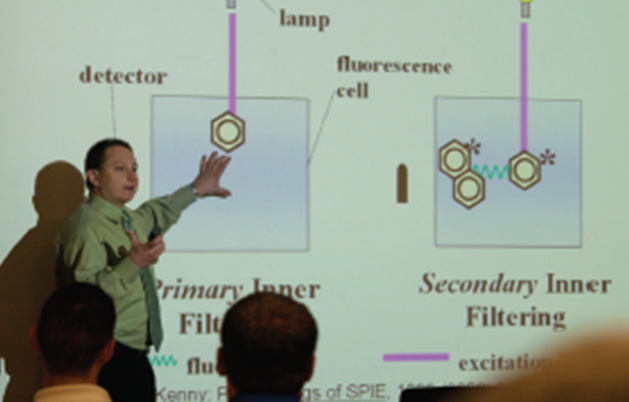
\includegraphics[width=\columnwidth]{Figure 1.jpg}
 \caption*{\textit{Credit: A. Sue Weisler, Rochester Institute of Technology/National Technical Institute for the Deaf (\url{www.rit.edu/NTID}).}}
    \label{Figure 1}
\end{figure}

\begin{enumerate}
    \item[D)] \textit{Graduates Obtaining Jobs}
    \begin{sloppypar}There is no question about it, money talks when evaluating the success of a program. After about two years of study and a 10-week co-op stint, has the program been worthwhile to its graduates? It has, if quality jobs in the field are obtainable by the graduates. Usually this is not much of a problem when the economy can absorb the graduates, but the challenge is when it cannot accommodate them. Programs are successes when graduates can obtain suitable jobs in economically bad times.

    Compared to their hearing counterparts, graduates of the LST program may have additional obstacles to overcome when finding a job. Employers naturally wonder how they will communicate with the deaf or hard-of-hearing employee. Safety issues in the laboratory workplace are concerns for potential employers who worry about how much supervision a deaf or hard-of-hearing employee might require. Graduates and faculty members alike must convince potential employers that deaf professionals have a long history of success in the workplace by giving examples and discussing their own co-op successes. In addition, the program’s reputation and the graduate’s skills set must be clear to potential employers. The program’s continued response to the needs of industry, hands-on/practical curriculum, and thorough training of its students must remain in tact in order to give our graduates a competitive advantage in the workplace.\end{sloppypar}
    \item[E)] \textit{Student Co-op Placement}
    \begin{sloppypar}A crucial aspect of the LST program is a required co-operative work experience/internship. As part of their graduation requirements, deaf and hard-of-hearing LST students must successfully complete at least 350 hours of a summer internship experience in an academic, government, or industrial setting. These internship opportunities are essential for preparing the students for future work experience, expanding their view of science, and providing an excellent setting for students to apply skills developed in the teaching classroom/laboratory. The deaf and hard-of-hearing students who complete the internship program tend to demonstrate great pride in their accomplishment, as well as observable personal and academic growth.

    Though it is not a requirement that the co-op is paid, in most cases companies do directly pay the students. Over the past few years, 80\% of the students that completed their co-op experience were paid. Using the co-op as a vehicle, students gain real-world technical experience, get a taste of the working world, and are able to affirm their choice of career focus. The program prides itself on their students’ ability to enter a host company’s laboratory and contribute from the start. Co-op employers often communicate their pleasure with the students’ preparedness, maturity, and competence. Many companies that hire our students are thrilled with the experience and many hire additional co-op students in subsequent years. The program has placed students with a variety of different companies. Some of the organizations with which LST students have completed co-op experiences are Kodak, Novartis Pharmaceuticals, Monroe County Medical Examiner’s Office, Strong Memorial Hospital, FDA, Ortho Clinical Diagnostics, Land-of-Lakes, Eli Lilly, Dow Chemical, Stanford University, Tufts University, James Madison University, University of Massachusetts-Amherst, and NOAA.

    Placing a deaf or hard-of-hearing student on co-op can involve many of the same obstacles that were mentioned above for graduates seeking permanent employment. Faculty members assist in the co-op process by helping the students to seek co-op positions and working one-on-one with potential employers in order to alleviate any hesitations that they might have about hiring a deaf or hard-of-hearing student. These interactions with potential co-op partners often involve an explanation of the students’ training/preparation, success stories of prior LST students in co-op, and a discussion related to working with deaf and hard-of-hearing students. Individuals are often quite open-minded to working with deaf and hard-of-hearing professionals once their questions are answered. There is no question that there is the need to convince members of industry that the hiring of students who have yet to complete an associate level degree program can make good business sense. Faculty members invest countless hours in working with potential co-op employers, taking advantage of every opportunity to network with working professionals, discuss the students’ skills with the scientific community, and promote the program through their activities and travels. Faculty present at conferences, disseminate articles/papers about the program, call on their professional contacts, and travel throughout the country to assist with the placement of co-op students.\end{sloppypar}
\end{enumerate}

\section*{CONCLUSION}
A decade after its implementation, the LST program is thriving. It is a program like any other, yet like no other—a seeming contradiction. It faces challenges similar to other quality chemical technology programs, but with one crucial programmatic difference—its student population is deaf and hard-of-hearing. Despite this distinction, the students in the program are held to the same high standards as any other students in similar programs. Through its cultivation of industrial partnerships, constant skills/curriculum assessment, creative pedagogy, and diligent faculty efforts, the program is able to sustain and grow. As a result students take pride in their program, future students are attracted to the program’s documented successes, and industrial professionals are willing to work with LST students and graduates. Resonating with the mission of NTID, the LST program strives to continue to provide deaf and hard-of-hearing student with quality technological and lifelong learning skills that will give our students competitive advantages in industry; a goal rooted deeply enough that it can be seen in the very core of the program’s development and daily operation.

\end{large}
\clearpage
\section*{REFERENCES}\par 

\leftskip 0.25in
\parindent -0.25in 
%%%

Amato, I. (2006). Silent Chemistry. Chemical \& Engineering News, 84(12), 53-56.\\

Bureau of Labor Statistics (2010-11). Outlook Occupational Handbook. Retrieved from \url{http://www.bls.gov/oco/ocos115.htm#outlook.}

Bureau of Labor Statistics (May, 2010). Occupational Employment and Wages. Retrieved from \url{http://www.bls.gov/oes/current/oes194031.htm.}

ChemTechLinks (2006). Critical Issues and Effective Practices in Chemistry-Based Laboratory Technology Education. Washington, DC.

Hofstader, R., \& Chapman, K. (1997). Foundations for Excellence in the Chemical Process Industries: Voluntary Industry Standards for Chemical Process Industries Technical Workers. Washington, D.C.: American Chemical Society U.S. Department of Education, Office of Educational Research and Improvment, Educational Resources Information Center.

Huber, J. (2012). ACS Award for Encouraging Disadvantaged Students into Careers in the Chemical Sciences. Chemical \& Engineering News, 90, 41-42.

Hunt, C. T. (2007). All Aboard The Innovation Train! Chemical \& Engineering News, 85, 35.

The National Center for Higher Education Management Systems. (2009). Three-Year Graduation Rates for Associate Students. Retrieved from \url{http://www.higheredinfo.org/dbrowser/index.php?submeasure=24\&year=2009\&level=nation\&mode=graph\&state=0}

National Technical Institute for the Deaf (2011). 2011 Annual Report. Rochester, NY.

Pagano, T. (2009). Conducting Research with Early Undergraduates and Students with Special Needs. In Boyd \& Wesemann (Eds.), Broadening Participation in Undergraduate Research: Fostering Excellence and Enhancing the Impact. Washington, DC: Council on Undergraduate Research (CUR).

Pagano, T., \& Quinsland, L. K. (2007). Pedagogical Applications of Instant Messaging Technology for Deaf and Hard-of-Hearing Students in the Science Classroom. Journal of Science Education for Students with Disabilities, 12(1), 33-46.

Pagano, T., \& Quinsland, L. K. (2007). Pedagogical Applications of Instant Messaging Technology for Deaf and Hard-of-Hearing Students in the Science Classroom. Journal of Science Education for Students with Disabilities, 12(1), 33-46.

\end{document}
